\section{Infrastructure}
Deux types d'infrastructures seront disponibles:
\begin{itemize}
\item Infrastructure web, hébergé sur un serveur en ligne qui nous appartient.
\item Infrastructure web, hébergé sur une VM chez le client.\\
\end{itemize}

Alternatives non choisies:
\begin{itemize}
\item Client lourd: Contrainte d'installation pour l'utilisateur. Informations accessibles seulement depuis une seule machine.
\item Application mobile: pas très professionnel, moins simple d'utilisation.
\end{itemize}

\begin{figure}[!h]
  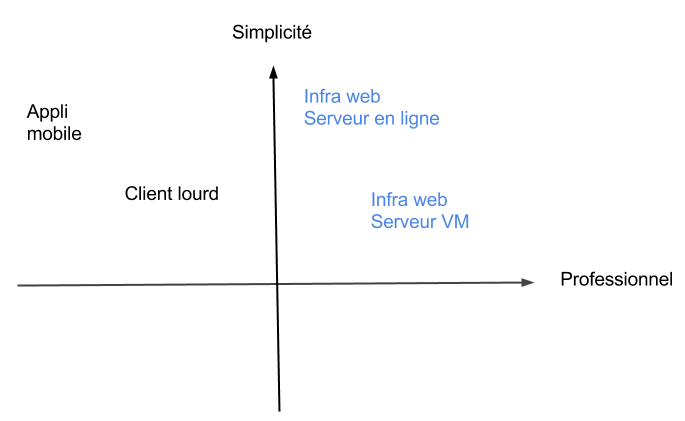
\includegraphics[width=18cm]{choix-infra.png}
\end{figure}

\newpage


\section{Composants logiciels}
Afin de choisir les différents composants logiciels du projet, nous nous sommes basés sur plusieurs critères :

Est-ce que la technologie est innovante ? Est-elle en constante évolution et nous permet-elle d'être en phase avec les autres choix du projet ?
La sécurité : est-ce que l'outil est pensé/orienté vers la sécurité, qu'elle soit de l'infrastructure ou du client ?
La rapidité de déploiement, de compréhension et d'exécution du composant : est-il facile à prendre en main, efficace ? Est-ce que la courbe d'apprentissage du composant correspond effectivement à nos besoins et à l'évolution du projet ?

\small
\begin{tabular}{| >{\raggedright}p{2.6cm}| >{\raggedright}p{3.5cm}| >{\raggedright}p{2cm}|p{7cm}|}
  \hline
  \rowcolor{Gainsboro}
  \color{Navy}{\bfseries{Choix des technologies Domaines}} & \color{Navy}{\bfseries{Technologies disponibles}} & \color{Navy}{\bfseries{Choix Vigilate}} & \color{Navy}{\bfseries{Justification}}\\
  \hline
  Framework Web & Ruby On Rails, Django, Symphony & Django & Innovant, En évolution, Orienté sécurité, En phase avec le langage de développement, Léger \\
  \hline
  Framework Javascript & jQuery, AngularJS & AngularJS & Complémentaire à Django Constante Evolution \\
  \hline
  Serveur HTTP & Apache, Nginx, Lighthttpd & Nginx & Performant, Léger \\
  \hline
  Langage de programmation & Ruby, Python, PHP & Python & Mise en place rapide, Grande flexibilité, Mutliplate-forme \\
  \hline
  Virtualisation & VmWare, VirtualBox, XEN & VirtualBox & OpenSource, Simple d’utilisation, Personnalisable \\
  \hline
  Base de données & MySQL, MariaDB, Sqlite, PostgreSQL & MariaDB, PostgreSQL & OpenSource, Simple d’utilisation, Générique\\
  \hline
\end{tabular}
\normalsize

\section{Multi OS et Multi DB}
N/A
\section{Mobile}
N/A